\documentclass[11pt,a4paper]{article}

% -----------------------------------------------------------------------------
% Paquetes
% -----------------------------------------------------------------------------
\usepackage[utf8]{inputenc}
\usepackage{enumitem}
\usepackage{amsmath}
\usepackage{amssymb}
\usepackage{booktabs}
\usepackage[T1]{fontenc}
\usepackage{tabularx} 
\usepackage{array}    
\usepackage{float}    
\usepackage{graphicx}
\usepackage{xcolor}
\usepackage{fancyhdr}
\usepackage[a4paper,margin=2.5cm,headheight=48pt]{geometry}

% Configuración del paquete caption para textos en gris claro:
\usepackage{caption}
\DeclareCaptionFont{grisclaro}{\color{black!45}} 
\captionsetup{font=grisclaro, labelfont={bf,grisclaro}} % Todo el caption en gris claro

% Fecha en español
\newcommand{\FechaEnEspanol}{%
  \number\day\space de\space
  \ifcase\month
    \or enero\or febrero\or marzo\or abril\or mayo\or junio\or
    julio\or agosto\or septiembre\or octubre\or noviembre\or diciembre
  \fi\space de\space\number\year
}

% lastpage
\newif\ifHayUltimaPagina
\IfFileExists{lastpage.sty}{
  \usepackage{lastpage}
  \HayUltimaPaginatrue
}{
  \HayUltimaPaginafalse
}

% -----------------------------------------------------------------------------
% CONFIGURACION DEL TRABAJO
% -----------------------------------------------------------------------------
\newcommand{\NombreMateria}{Redes de Computadoras}
\newcommand{\TipoTrabajo}{Trabajo Práctico}
\newcommand{\NumeroTrabajo}{5}
\newcommand{\TipoTP}{Práctico}
\newcommand{\NombreTrabajo}{Transmisión de Datos: de ICMP y ARP a Sockets TCP}
\newcommand{\NombreGrupo}{NetRunners}
\newcommand{\Docente}{SANTIAGO MARTIN HENN}
\newcommand{\LogoArchivo}{logo.png}
\newcommand{\LogoRuta}{\LogoArchivo}

\newcommand{\Integrantes}{%
  \begin{tabular}{ll}
    Bastida, Lucas Ramiro & DNI 39444511 \\
    Contessi, Ruben Andres & DNI 33315235 \\
    Garay, Ignacio Hernan & DNI 44191925 \\
    Giraudo, Juan Pablo & DNI 34970089 \\
    Peñaloza, Gonzalo Adrian & DNI 40441355 \\
    Quinteros del Castillo, Tomás Agustín & DNI 46169739 \\
    Vasconsellos Blason, Benjamin Alejandro & DNI 45642879 \\
  \end{tabular}%
}

\newcommand{\InsertarLogo}[1][0.24\textwidth]{%
  \ifx\LogoRuta\empty
    \fbox{\parbox[c][1cm][c]{#1}{\centering Logo institucional\\\small (colocar archivo)}}%
  \else
    \includegraphics[width=#1,keepaspectratio]{\LogoRuta}%
  \fi
}

\newcommand{\TituloCorto}{TP \NumeroTrabajo (\TipoTP): \NombreTrabajo}

\pagestyle{fancy}
\fancyhf{}
\fancyhead[L]{\InsertarLogo[1.2cm]}
\fancyhead[C]{\parbox{0.62\textwidth}{\centering\scriptsize\textbf{\TituloCorto}}}
\fancyhead[R]{\small\NombreGrupo}
\renewcommand{\headrulewidth}{0.4pt}
\fancyfoot[C]{\small Pagina \thepage\ifHayUltimaPagina\ de \pageref{LastPage}\fi}
\renewcommand{\footrulewidth}{0pt}

\begin{document}

\begin{titlepage}
  \thispagestyle{empty}
  \begin{center}
    \InsertarLogo[0.32\textwidth]

    \vfill
    {\Large\textsc{\NombreMateria}\par}
    \vspace{1.5cm}
    {\Huge\bfseries \TipoTrabajo\par}
    \vspace{0.35cm}
    {\LARGE N.\textsuperscript{o} \NumeroTrabajo (\TipoTP)\par}
    \vspace{0.8cm}
    {\Large\NombreTrabajo\par}

    \vfill
    \begin{tabular}{rl}
      \textbf{Grupo:} & \NombreGrupo \\
      \textbf{Docente:} & \Docente
    \end{tabular}

    \vspace{1cm}
    \begin{center}
      \textbf{Integrantes}\\[0.2cm]
      \Integrantes
    \end{center}

    \vfill
    {\large \FechaEnEspanol\par}
  \end{center}
\end{titlepage}


%% Punto 1)

\section*{1) ICMP y primer contacto con Wireshark} 

\begin{enumerate}[label=\alph*)]

\item
    ICMP (Internet Control Message Protocol) es un protocolo auxiliar de la capa de red (Capa 3 del modelo OSI / Capa Internet de TCP/IP). Se utiliza para transmitir mensajes de control, diagnóstico, reporte de errores y pruebas de alcanzabilidad entre dispositivos de red (hosts y routers). ¿Transporta datos de aplicaciones? No. A diferencia de TCP o UDP, ICMP no está destinado al transporte de datos de usuario/aplicación final (como la navegación web, archivos o correo), sino al control y diagnóstico de la propia infraestructura de red.
\item
    El protocolo ICMP trabaja en la capa de red, pero viaja empaquetado/encapsulado dentro de IP. El receptor analiza el campo Protocol (Protocolo) de la cabecera IP. Cuando el valor de este campo es 1, la capa IP sabe que el payload (carga útil) contenido en el paquete IP es un mensaje ICMP.
\item
    ping es una herramienta de software que utiliza ICMP para verificar si un host destino es alcanzable a través de la red y medir el tiempo de ida y vuelta (Round Trip Time o RTT). Los campos que los distinguen son: Type (Tipo) y Code (Código) del encabezado ICMP.
\item
    Un mensaje ICMP tipo Echo contine:

    \begin{itemize}
        \item Type (1 byte): Identifica si es Request (8) o Reply (0).
        \item Code (1 byte): Subcódigo (generalmente 0 para Echo).
        \item Checksum (2 bytes): Para verificación de errores en la cabecera e información ICMP.
        \item Identifier (ID - 2 bytes): Para asociar solicitudes y respuestas en un proceso/proceso ping.
        \item Sequence Number (2 bytes): Número de secuencia para asociar cada Request específico con su Reply correspondiente.
        \item Data / Payload: Datos opcionales/de relleno (timestamps, secuencias de texto o números) enviados para calcular los tiempos y verificar que los datos lleguen intactos.
    \end{itemize}

    \begin{figure}[H]
      \centering
      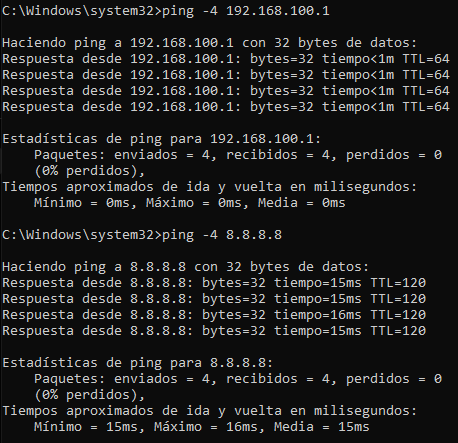
\includegraphics[width=\linewidth]{pings.png}
      \caption{Pings Gateway - 8.8.8.8}
      \label{fig:captura_consola}
    \end{figure}

    \begin{figure}[H]
      \centering
      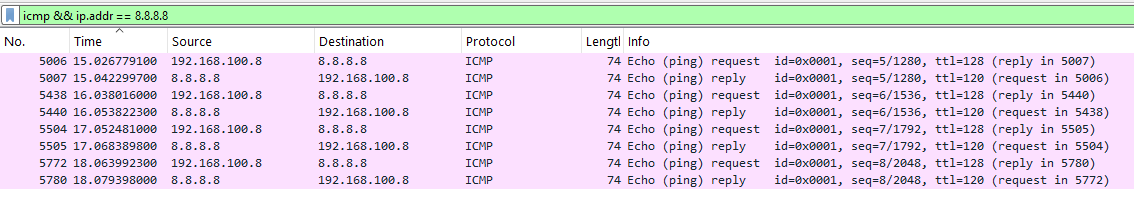
\includegraphics[width=\linewidth]{wire.png}
      \caption{Captura WireShark con Filtro}
      \label{fig:captura_wireshark}
    \end{figure}

\begin{table}[h!]
\centering
\renewcommand{\arraystretch}{1.8}
\begin{tabularx}{\textwidth}{|>{\raggedright\arraybackslash}p{3.8cm}|X|X|>{\raggedright\arraybackslash}p{4cm}|}
\hline
\textbf{Capa (como la nombra Wireshark)} & \textbf{Origen} & \textbf{Destino} & \textbf{¿Qué campo indica qué protocolo viene "adentro"?} \\ \hline
Ethernet II & fc:4d:a6:cd:4c:32 & e0:d5:5e:2a:5e:ee & Type \\ \hline
Internet Protocol Version 4 & 192.168.100.8 & 8.8.8.8 & Protocol \\ \hline
Internet Control Message Protocol & Identifier (BE) = 1 (0x0001) & Identifier (BE) = 1 (0x0001) & Type / Code   \\ \hline
Datos / payload & N/A & N/A & N/A \\ \hline
\end{tabularx}
\end{table}

\item
    \leavevmode
    \begin{figure}[H]
      \centering
      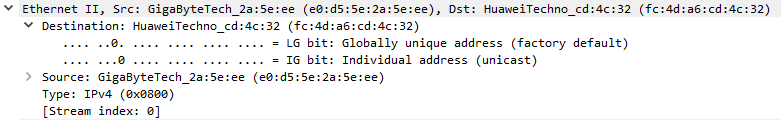
\includegraphics[width=\linewidth]{echoReq.png}
      \caption{Echo Request 8.8.8.8}
      \label{fig:captura_wireshark1}
    \end{figure}

    No, no es la MAC de 8.8.8.8. Es la dirección MAC de nuestro propio Router. 

    \begin{figure}[H]
    \centering
    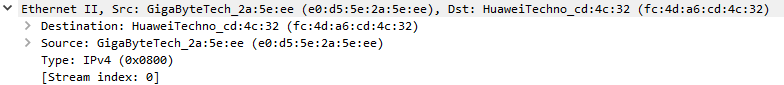
\includegraphics[width=\linewidth]{echoReqGat.png}
    \caption{Echo Request al gateway}
    \label{fig:captura_wireshark2}
    \end{figure}

    Como podemos observar en el echo Request al gateway, la dirección MAC de destino es la del router. De esto podemos concluir que el alcance de la direccion MAC es puramente local mientras que el alcance de la direccion IP es global por lo que para enviar un paquete a una dirección IP que no se encuentra en la misma red local, el paquete debe ser enviado al router, que se encargará de reenviarlo a su destino.

\item
    Los campos que cambian son:
    \begin{itemize}
        \item \textbf{Ethernet II:}
        \begin{itemize}
            \item Source y Destination MAC Address: En este caso tiene sentido ya que uno es de request y el otro de reply, por lo que el sentido de flujo de datos se invierte.
        \end{itemize}
        \item \textbf{IPv4:}
        \begin{itemize}
            \item Identification: El identificador del paquete IP cambia en cada paquete enviado por la pila de red.
            \item Source y Destination IP Address: Al igual que en el caso anterior, tiene sentido que se inviertan.
            \item Time to Live (TTL).
            \item Header Checksum: Cambia porque el TTL cambió, y el checksum se calcula sobre el header del paquete IP.
        \end{itemize}
        \item \textbf{ICMP:}
        \begin{itemize}
            \item Type: Cambia de 8 (echo request) a 0 (echo reply).
            \item Checksum: Cambia porque el tipo cambió, y el checksum se calcula sobre todo el paquete ICMP.
        \end{itemize}
    \end{itemize}

    Los campos que se mantienen igual son:
    \begin{itemize}
        \item \textbf{IPv4:} Version, Header Length, Protocol.
        \item \textbf{ICMP:} Identifier, Sequence Number.
    \end{itemize}

    Los campos identifier y sequence number se mantienen iguales porque le permiten a la herramienta ping asociar inequívocamente cada Echo Reply que llega con el Echo Request específico que envió previamente, calculando así el tiempo de ida y vuelta (RTT) exacto de cada paquete.

\item
    Se encuentra ubicado al final de la trama, como la carga útil empaquetada dentro del encabezado del protocolo ICMP. Tiene un tamaño de 32 bytes y contiene un patrón de bytes de relleno que consiste en una secuencia alfabética repetitiva de texto en formato ASCII y además es exactamente igual en el Reply. 
    
    \begin{figure}[H]
    \centering
    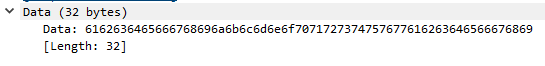
\includegraphics[width=\linewidth]{payload.png}
    \caption{Payload del paquete ICMP.}
    \label{fig:payload_icmp}
    \end{figure}

    Windows utiliza 32 bytes de letras ASCII mientras que Linux suele enviar 56 bytes incluyendo una marca de tiempo timestamp. Esto demuestra que la norma ICMP no exige un estándar fijo de contenido para el payload de prueba; cada sistema operativo implementa su propio generador de datos según el software ejecutable ping.

\item
    El echo request tiene un valor de Time to Live (TTL) de 128 y el del reply 120. Esto se debe a que cada router intermediario en Internet descuenta 1 unidad al campo TTL del paquete IP para evitar bucles de enrutamiento, dado que la respuesta enviada desde el servidor 8.8.8.8 se genera con un TTL = 128 el valor final recibido de 120 nos indica que la trama atravesó 8 saltos de routers intermedios hasta llegar de regreso a nuestro equipo. 

\item \leavevmode
    \begin{figure}[H]
    \centering
    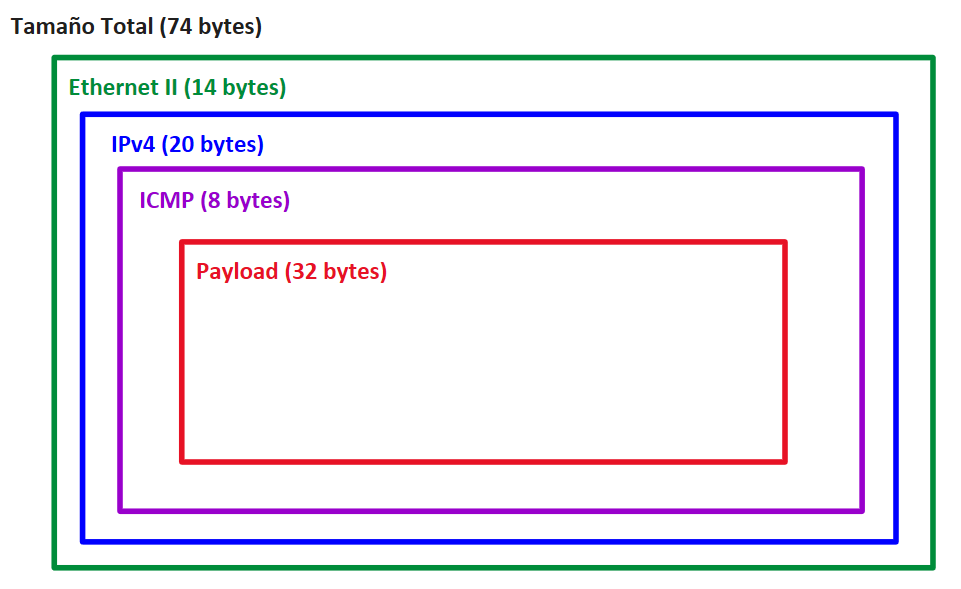
\includegraphics[width=\linewidth]{boxes.png}
    \caption{Encapsulado del paquete.}
    \label{fig:encapsulado}
    \end{figure}

\end{enumerate}

\vspace{0.8cm}
\section*{2) ARP: de una IP a una dirección MAC} 

\begin{enumerate}[label=\alph*)] 

\item 
\item 
\item 
\item 
\item 
          

\end{enumerate}


\section*{3) TCP y UDP a mano con ncat} 

\subsection*{Conceptos previos}

\begin{enumerate}[label=\alph*)]

\item \textbf{¿Qué significa establecer una conexión? ¿Dónde existe una conexión TCP?}

Establecer una conexión TCP significa realizar un intercambio inicial de segmentos entre los extremos para iniciar la comunicación. Este establecimiento se realiza mediante tres pasos: SYN, SYN-ACK y ACK. La conexión es una asociación lógica entre los extremos, no algo que exista en los cables o routers.

\item \textbf{¿Qué es un puerto? ¿Qué identifica el par (IP, puerto)?}

Un puerto es un punto de acceso que permite identificar un proceso o servicio dentro de un equipo. El par (IP, puerto) permite identificar un extremo de comunicación, indicando el equipo y el proceso o servicio al que se dirige el tráfico.

\item \textbf{¿Qué significa que un proceso esté escuchando en un puerto?}

Significa que el proceso está preparado para recibir comunicaciones dirigidas a ese puerto. En TCP, el servidor espera solicitudes de conexión de los clientes para poder establecer una conexión y comenzar el intercambio de datos.

\end{enumerate}

\subsection*{Experimento TCP}

Se ejecutó un servidor con \texttt{ncat} escuchando en el puerto TCP 12000 y un cliente que se conectó a la dirección \texttt{127.0.0.1}. La captura se realizó con Wireshark utilizando el filtro \texttt{tcp.port == 12000}.

En la captura se identificaron las siguientes etapas:

\begin{itemize}
  \item \textbf{Establecimiento de la conexión:} se observan los segmentos SYN, SYN-ACK y ACK, que conforman el establecimiento de la conexión TCP.
  \item \textbf{Intercambio de datos:} aparecen segmentos con las banderas PSH y ACK que transportan los mensajes enviados entre el cliente y el servidor. También se observan segmentos ACK sin datos de aplicación.
  \item \textbf{Cierre de la conexión:} se identifican segmentos FIN-ACK y ACK que intervienen en el cierre de la conexión.
\end{itemize}

\begin{figure}[H]
  \centering
  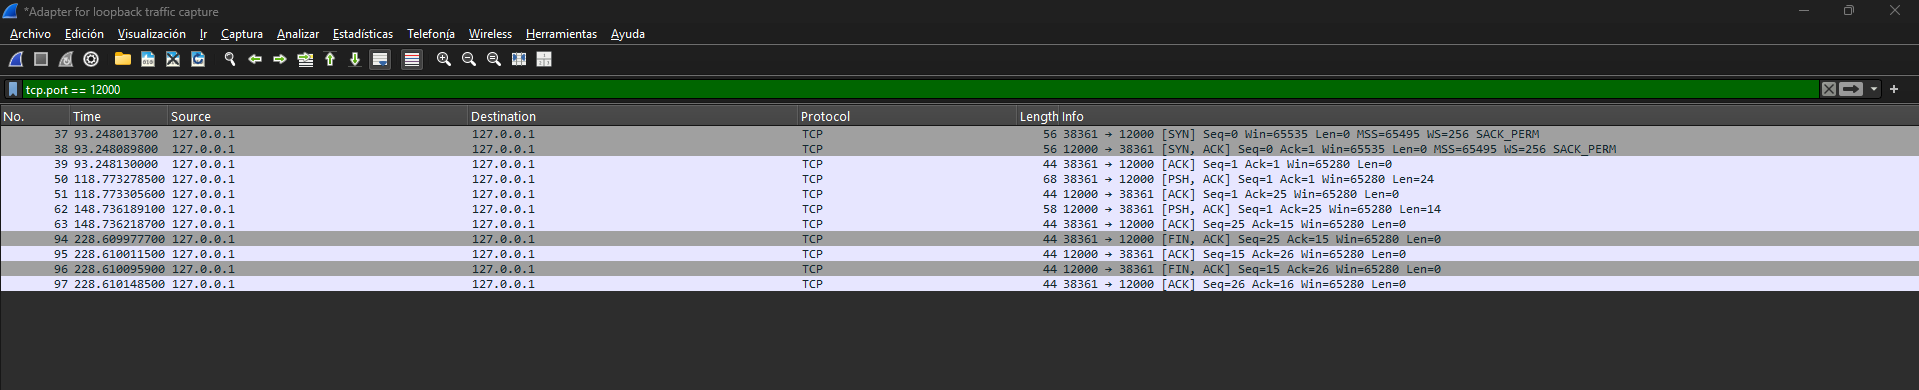
\includegraphics[width=\textwidth]{Experimento_TCP}
  \caption{Captura del intercambio TCP con Wireshark.}
  \label{fig:experimento-tcp}
\end{figure}

\subsection*{Experimento UDP}

Se realizó una comunicación UDP utilizando el puerto 12001. El servidor quedó a la espera de datagramas y el cliente envió el mensaje ``Hola servidor''. Luego, el servidor respondió con el mensaje ``Hola cliente''. El tráfico se capturó con Wireshark.

\begin{figure}[H]
  \centering
  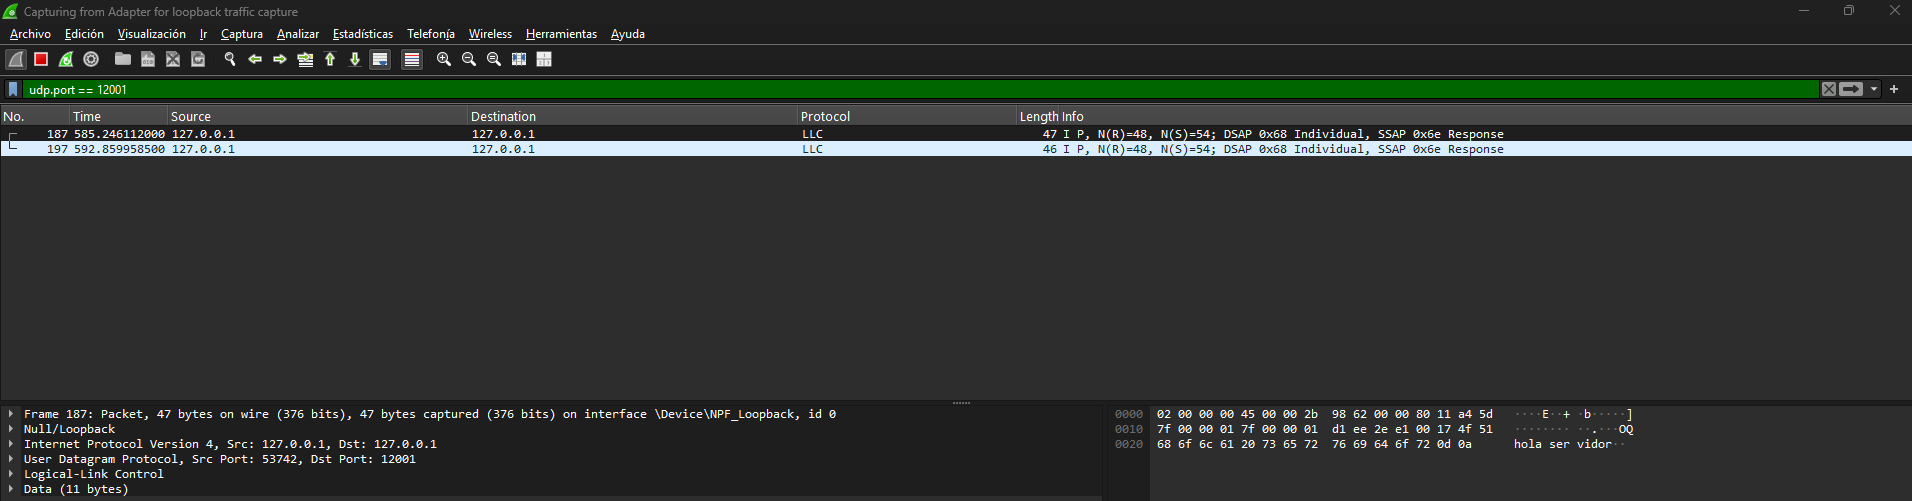
\includegraphics[width=\textwidth]{udp_cliente_servidor.png}
  \caption{Datagrama UDP enviado desde el cliente al servidor.}
  \label{fig:udp-cliente-servidor}
\end{figure}

En esta captura se observa un datagrama con puerto de origen 53742 y puerto de destino 12001. Los datos transmitidos ocupan 11 bytes y corresponden al mensaje ``Hola servidor''.

\begin{figure}[H]
  \centering
  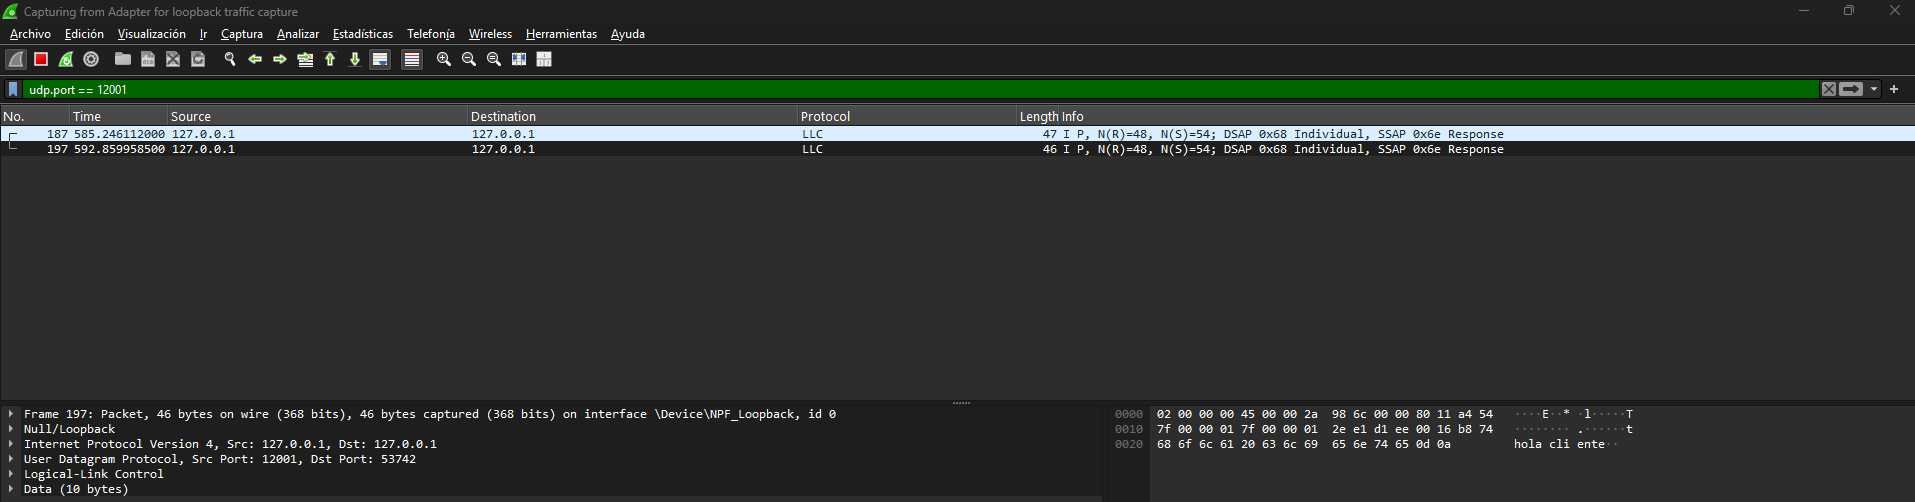
\includegraphics[width=\textwidth]{udp_servidor_cliente.png}
  \caption{Datagrama UDP enviado desde el servidor al cliente.}
  \label{fig:udp-servidor-cliente}
\end{figure}

En esta captura se observa el sentido inverso: el puerto de origen es 12001 y el puerto de destino es 53742. Los datos transmitidos ocupan 10 bytes y corresponden al mensaje ``Hola cliente''.

En ambas capturas, aunque la columna \textit{Protocol} de Wireshark muestra LLC, el panel de detalles permite identificar los encabezados IPv4 y UDP, junto con los puertos de origen y destino.

\subsection*{Comparación entre TCP y UDP}

\begin{enumerate}[label=\alph*)]

\item Antes de enviar el primer mensaje, UDP no necesita establecer una conexión. En cambio, TCP realiza un intercambio inicial de tres segmentos (SYN, SYN-ACK y ACK) antes de transmitir los datos.

\item En la captura UDP, cada uno de los mensajes observados se transmite en un datagrama independiente. No se observan confirmaciones ACK propias de UDP. En TCP, en cambio, se observan segmentos de confirmación durante el intercambio de datos.

\item Comparación de las cabeceras TCP y UDP.

La cabecera TCP observada en Wireshark tiene un tamaño de
20 bytes (160 bits), mientras que la cabecera UDP tiene un
tamaño fijo de 8 bytes (64 bits). Ambos protocolos incluyen
los puertos de origen y destino. TCP incorpora además campos
como números de secuencia, confirmación y banderas de control,
mientras que UDP posee una cabecera más simple, con campos
de longitud y suma de comprobación.

\begin{figure}[H]
  \centering
  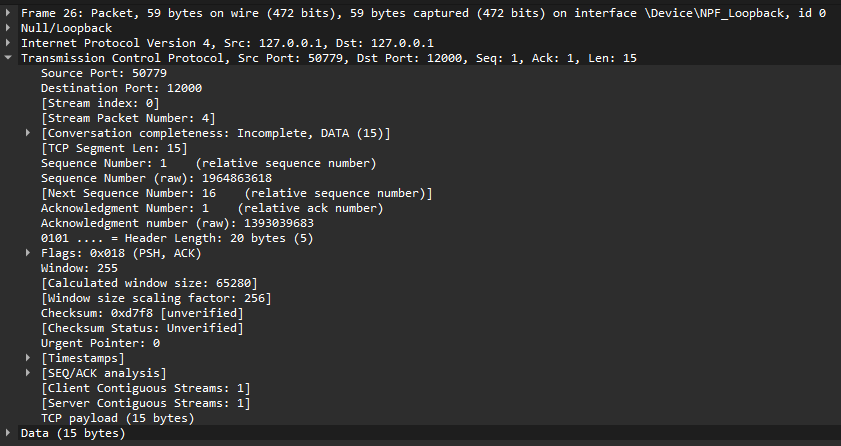
\includegraphics[width=0.9\textwidth]{tcp_cabecera.png}
  \caption{Detalle de la cabecera TCP en Wireshark.}
  \label{fig:tcp-cabecera}
\end{figure}

\begin{figure}[H]
  \centering
  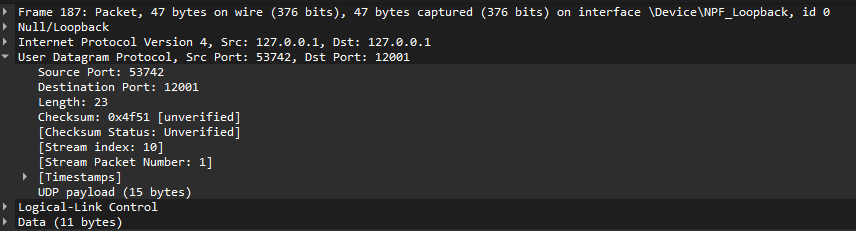
\includegraphics[width=0.9\textwidth]{udp_cabecera.png}
  \caption{Detalle de la cabecera UDP en Wireshark.}
  \label{fig:udp-cabecera}
\end{figure}

\item Al cerrar el cliente UDP con Ctrl+C, no se realiza un
intercambio de mensajes de cierre, ya que UDP no establece
una conexión. En cambio, al cerrar la conexión TCP se
observa un intercambio de segmentos FIN y ACK para finalizar
la comunicación de forma ordenada.

\item \leavevmode % Completar con el conteo de paquetes capturados al enviar
En ambas pruebas se envió el mensaje ``hola'' desde el cliente
hacia el servidor.

En la captura TCP se observan 9 paquetes en total: 3 para
establecer la conexión, 2 correspondientes al envío del mensaje
y su confirmación, y 4 para cerrar la conexión. En la captura
UDP se observa un datagrama para enviar el mensaje.

Los paquetes adicionales de TCP permiten establecer y cerrar
la conexión, además de confirmar la recepción de los datos.
Estos mecanismos contribuyen a ofrecer una comunicación
confiable y ordenada, mientras que UDP no requiere establecer
una conexión ni utiliza confirmaciones de recepción propias
del protocolo.

\begin{figure}[H]
  \centering
  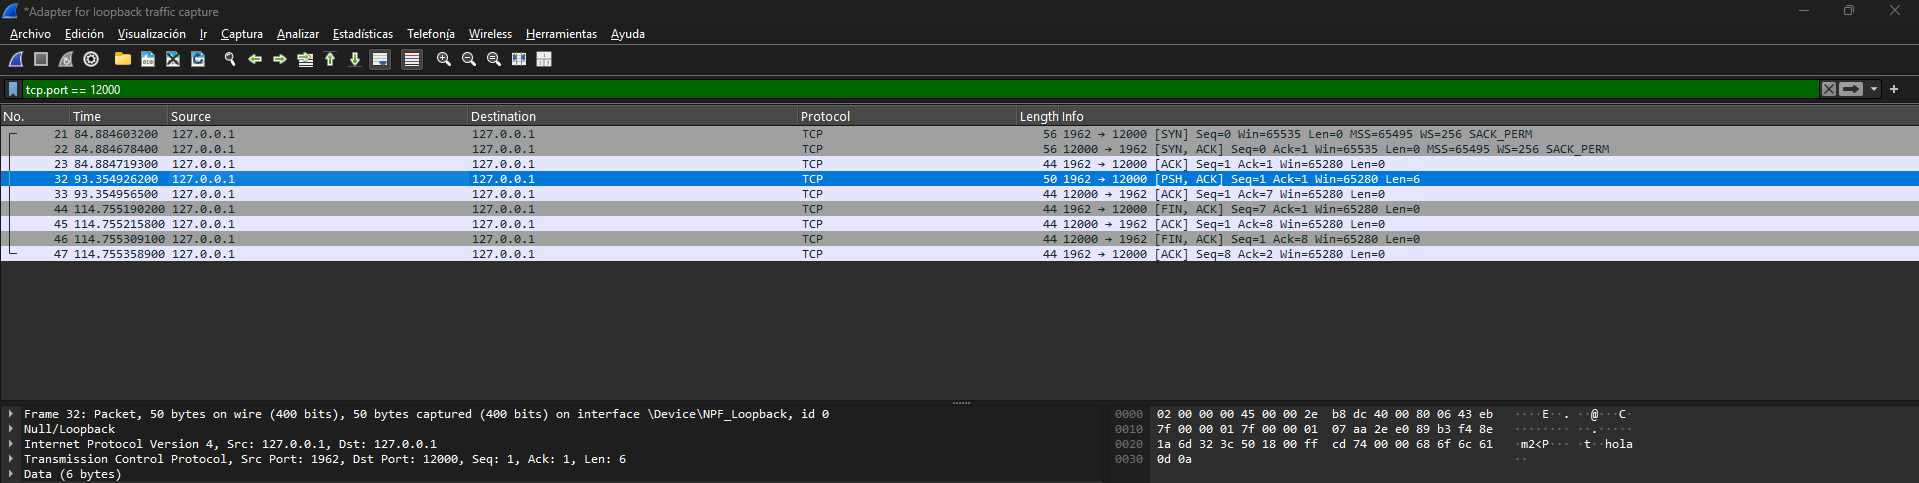
\includegraphics[width=0.9\textwidth]{tcp_pt_3e.png}
  \caption{Captura TCP del envío del mensaje ``hola'' desde
  el cliente al servidor, incluyendo el establecimiento y
  el cierre de la conexión.}
  \label{fig:tcp-punto-e}
\end{figure}

\begin{figure}[H]
  \centering
  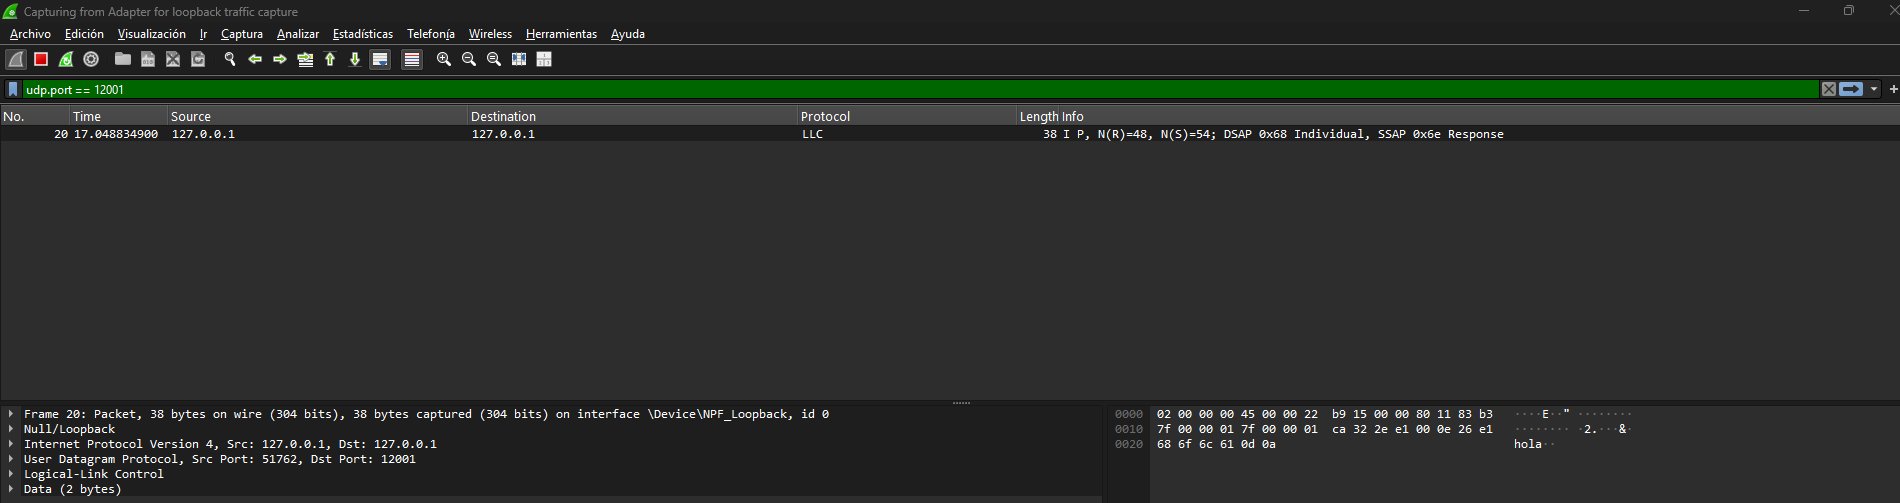
\includegraphics[width=0.9\textwidth]{udp_pt_3e.png}
  \caption{Captura UDP del envío del mensaje ``hola'' desde
  el cliente al servidor.}
  \label{fig:udp-punto-e}
\end{figure}

\item \leavevmode % Completar después de realizar la prueba sin servidores escuchando
Al intentar establecer una conexión TCP con el puerto 12000,
el cliente envía segmentos SYN y recibe respuestas RST, ACK,
indicando que la conexión es rechazada porque no hay ningún
proceso escuchando en ese puerto.

En el caso de UDP, el cliente puede enviar un datagrama al
puerto 12001 sin establecer previamente una conexión. Como
no hay ningún proceso escuchando en ese puerto, se recibe un
mensaje ICMP \textit{Destination unreachable (Port
unreachable)}, que indica que el puerto de destino no está
disponible.

\begin{figure}[H]
  \centering
  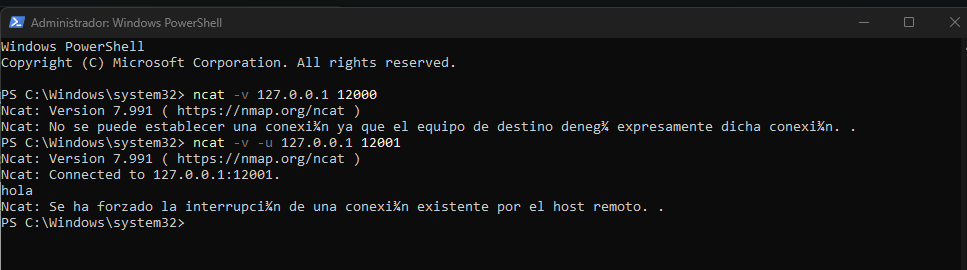
\includegraphics[width=0.85\textwidth]{pws_pt_3f.png}
  \caption{Salida de PowerShell al intentar comunicarse con
  los puertos TCP y UDP sin un servidor escuchando.}
  \label{fig:powershell-punto-f}
\end{figure}

\begin{figure}[H]
  \centering
  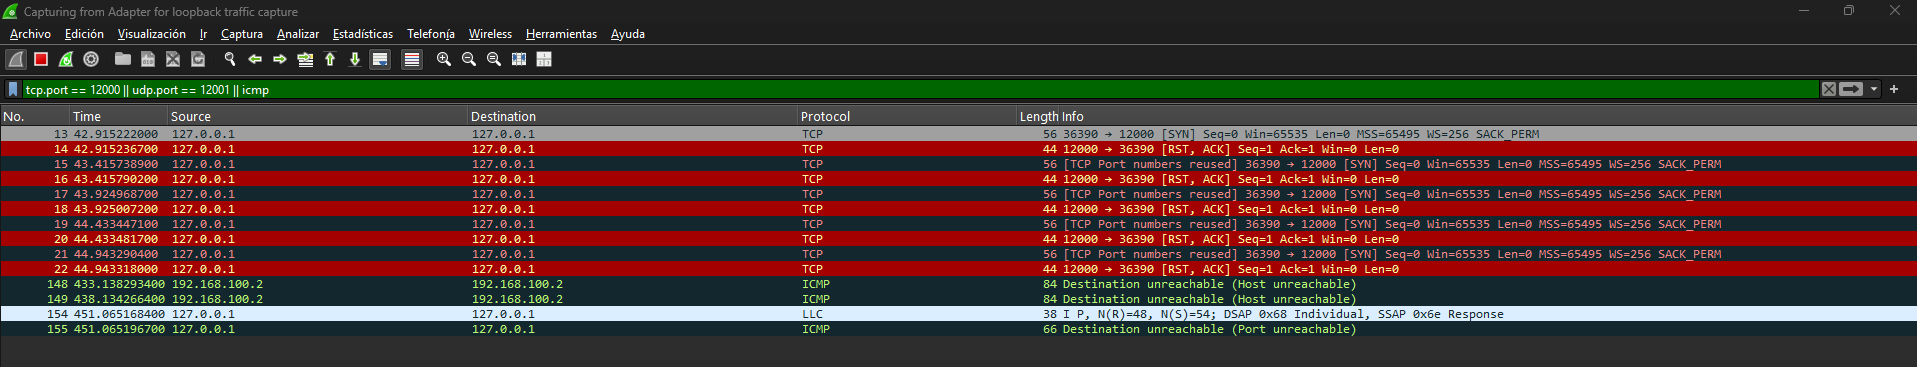
\includegraphics[width=\textwidth]{ws_pt_3f.png}
  \caption{Captura de Wireshark con los intentos de conexión
  TCP y el mensaje ICMP de puerto UDP inaccesible.}
  \label{fig:wireshark-punto-f}
\end{figure}

\end{enumerate}


\section*{4) Servidor TCP minimo} 

\begin{enumerate}[label=\alph*)] 

\item 

          

\end{enumerate}

\end{document}